\chapter[Conclusion and Future Work]{Conclusion and Future Work}
\chaptermark{Conclusion}
\label{chap:conclusion}
\minitoc

\subsection{Marker-free Unified Eye-hand Calibration}
\chapref{chap:registration}
- differentiable rendering -> solving draped robots

\subsection{Visual Servo}
\chapref{chap:robotic_endoscope}
- QP or other solvers

\subsection{Homography Estimation}
\chapref{chap:camera_motion_extraction}
- novel view synthesis
    - runtime for data
    - no diffusion models \cite{rombach2022high} as these tend to hallucinate and iterative  
\begin{figure}
    \centering
    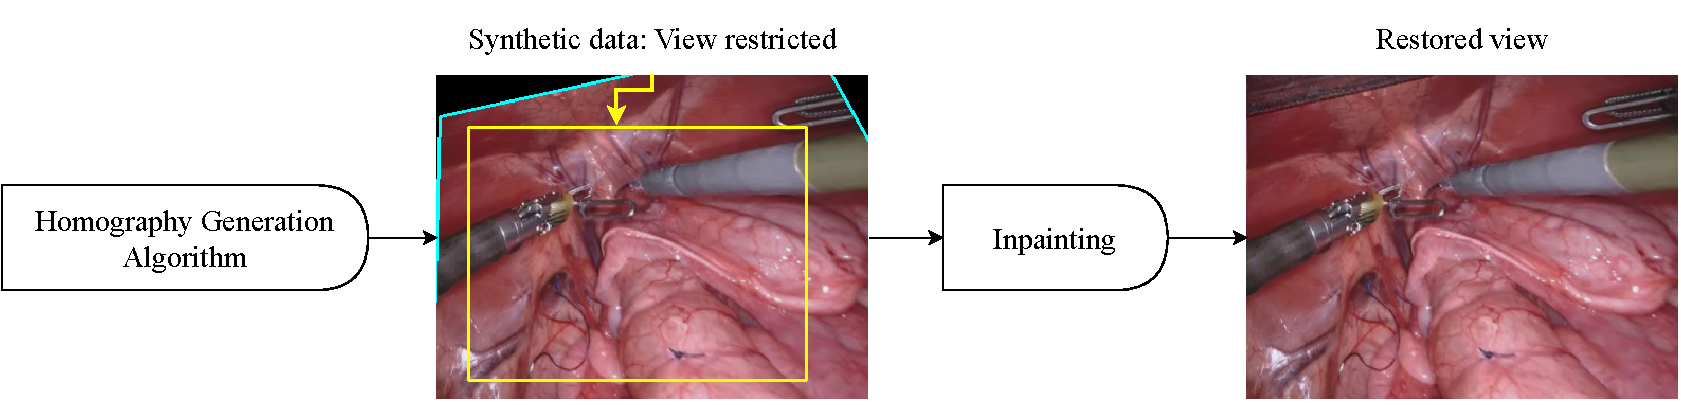
\includegraphics[width=\textwidth]{conclusion/fig/fourier_inpainting.pdf}
    \caption{Algorithm from \secref{c3:sec:hom_gen} \figref{c3:fig:hom} Caption \cite{suvorov2021resolution}.}
    \label{con:fig:inpainting}
\end{figure}
- incorporate depth \cite{budd2024transferring}: novel view synthesis
- utilize inpainting methods as well
- inpainting -> better range


\subsection{Homography Prediction}
\chapref{chap:camera_motion_prediction}

- rl on-top (force controlled rcm, rlhf)
- bootstrapping motion:
    - visual qa
- llm interface models

\subsection{Other Stuff}



% My thesis showed I did very useful things and also pleases my supervisor~\cite{Ourselin:MICCAI:00}. I also showed that I somewhat address the challenges laid out in \chapref{chap:intro}.
